% ===========================================================================
% main.tex -- the manuscript, in the PoPETs 2027 template.
%
% Supersedes paper/reference_draft.tex. Same evidence, revised for clarity
% and moved into the venue template; see paper/CHANGELOG.md.
%
% The "anonymous" class option is REMOVED per author instruction. Restore it
% (\documentclass[sigconf,anonymous,review]{acmart}) before any anonymous
% submission, or the author block will be visible to reviewers.
% ===========================================================================
\documentclass[sigconf,review]{acmart}

% popets.sty ships with the venue template and is not on this machine. The
% guard lets the manuscript compile locally; inside the real template the
% package loads normally. DO NOT remove the \usepackage line.
% \makeatletter must be OUTSIDE the conditional: \IfFileExists reads both
% branches as arguments, so the catcode of @ is fixed at read time.
\makeatletter
\IfFileExists{popets.sty}{%
  \usepackage{popets}%
  \setcopyright{popets}%
}{%
  \PackageWarningNoLine{main}{popets.sty not found: compiling with local
    stubs. Build inside the PoPETs 2027 template before submitting}%
  \@ifundefined{ethics}{\newenvironment{ethics}{\section*{Ethical Considerations}}{}}{}%
  \@ifundefined{openscience}{\newenvironment{openscience}{\section*{Open Science}}{}}{}%
  \@ifundefined{ai}{\newenvironment{ai}{\section*{AI Use}}{}}{}%
}
\makeatother

\copyrightyear{YYYY}
\acmYear{YYYY}
\acmVolume{YYYY}
\acmNumber{X}
\acmDOI{XXXXXXX.XXXXXXX}
\acmISBN{}
% \settopmatter FIRST: acmart's \acmConference takes three mandatory arguments
% ([short]{name}{date}{venue}). Called with one, it silently swallows the next
% two groups -- which put the literal string "printacmref=false,..." into the
% running head. popets.sty normally supplies the venue line; the empty date
% and venue here are placeholders for the local build.
\settopmatter{printacmref=false,printccs=false,printfolios=true}
\acmConference[PoPETs]{Proceedings on Privacy Enhancing Technologies}{}{}

\usepackage{booktabs}
\usepackage{graphicx}
% Figures and tables are the validated package; rebuilding it updates the
% paper with no edits here.
\graphicspath{{../results/paper_package/figures/}{figures/}{./}}
\makeatletter
\providecommand\input@path{}
\g@addto@macro\input@path{{../results/paper_package/tables/}{tables/}}
\makeatother

% ---------------------------------------------------------------------------
% Notation macros (one definition each, so the paper is consistent).
% ---------------------------------------------------------------------------
\newcommand{\FJ}{\ensuremath{\mathrm{F1}_{J}}}
\newcommand{\FL}{\ensuremath{\mathrm{F1}_{L}}}
\newcommand{\bJ}{\ensuremath{b_{J}}}
\newcommand{\AJ}{\ensuremath{A_{J}}}
\newcommand{\Asch}{\ensuremath{A_{\mathrm{schema}}}}
\newcommand{\VJ}{\ensuremath{V_{J}}}
\newcommand{\VL}{\ensuremath{V_{L}}}
\newcommand{\AVJ}{\ensuremath{A_{VJ}}}
\newcommand{\AVL}{\ensuremath{A_{VL}}}
\newcommand{\posthoc}{\ensuremath{^{\dagger}}}
\newcommand{\sonnet}{\textsf{claude-sonnet-5}}
\newcommand{\TODO}[1]{\textbf{[TODO: #1]}}
% Long compounds that otherwise overflow a narrow acmart column.
\hyphenation{de-anon-y-mi-za-tion re-source-bound-ed re-con-struc-tion
  frag-men-ta-tion un-link-abil-i-ty gran-u-lar-i-ty mem-ber-ship}

\begin{document}

\title[Shards of Meaning]{Shards of Meaning: Reassembly Under LLM Adversaries}

\author{Aiden J. Tejada}
\affiliation{%
  \institution{Trinity College}
  \city{Hartford}
  \state{CT}
  \country{USA}}
\email{aiden.tejada@trincoll.edu}

\author{Michael Anyaegbunam}
\affiliation{%
  \institution{Georgia Institute of Technology}
  \city{Atlanta}
  \state{GA}
  \country{USA}}
\email{manyaegbunam3@gatech.edu}

\author{Mohammed Arafat Nadaf}
\affiliation{%
  \institution{Northeastern University}
  \city{Boston}
  \state{MA}
  \country{USA}}
\email{nadaf.m@northeastern.edu}

\renewcommand{\shortauthors}{Tejada et al.}

% ---------------------------------------------------------------------------
\begin{abstract}
Fragmentation, cutting records into pieces and withholding their order and
grouping, has been proposed as a privacy mechanism for stored data. Its
unlinkability argument assumes the pieces cannot be put back together. We ask
how much an adversary holding the plaintext pieces recovers.

We define two games on frozen, pre-registered pools. Game~J gives the attacker
every fragment of a pool of seven documents, shuffled and under masked
aliases, and asks for both source membership and within-source order; Game~O
supplies membership and asks only for order. Game~J is scored with an
ordered-pair F1 that decomposes exactly into a linkage component and a
conditional ordering component, so a failure can be attributed to one half.

On clinical case reports published after the attacker model's training cutoff,
a one-shot large language model reached $\FJ = 0.723$ on 46 full-length pools,
recovering most membership ($\FL = 0.882$) and most relative order
($q = 0.792$), against an analytic one-bucket reference of $0.149$ and a legal
random seven-group answer of $0.077$. That score measures precedence, not
contiguity: on the same pools immediate-adjacency F1 was $0.287$ and the mean
longest intact run was $4.53$ fragments. The attacker recovers source
association and broad relative order strongly; contiguous plaintext recovery
is much weaker. Tested statistical and embedding attackers stayed near their
references.

Resistance depended on what the fragments retained. Synthetic identifier
records behaved qualitatively differently: the record template was recovered
in every group, but fields were not associated across records and every tested
content-based attacker scored below a truth-free schema-order baseline. In a
post-hoc controlled arm over five cuts of identical text, null-adjusted
reconstruction fell monotonically from $\AVJ = 0.588$ at a sentence cut to
$0.016$ at one word. Our contribution is the measurement and its
decomposition rather than a new reassembly algorithm.
\end{abstract}

\keywords{fragmentation, reconstruction attacks, large language models,
document reassembly, data privacy}

\maketitle

% ===========================================================================
\section{Introduction}
\label{sec:intro}
% ===========================================================================

Fragmentation is a standard answer to a specific privacy problem. Some
information is sensitive not because any single value is secret but because the
\emph{association} between values is: a date of birth is not identifying, a
postcode is not identifying, and a diagnosis may be public, but the three
together may identify a patient. Splitting the data so that constrained
attributes never appear together in the clear, and encrypting what cannot be
split, is a well-developed design~\cite{ciriani2010}.

That design rests on an assumption with a known failure mode. Requiring
fragments to share no attributes is \emph{necessary but not sufficient} for
unlinkability, because dependencies among the data may allow the fragments to
be recombined~\cite{decapitani2014}. That result is formulated for declared,
attribute-level dependencies supplied to the protection design as inputs.

We ask what happens when the relationship is not declared and not expressible
in that form---when it is simply what the text says. Our question is empirical:
do the implicit relationships carried by unconstrained plaintext constitute a
comparable reconstruction channel for a modern generative attacker?

Fragmentation withholds two distinct things, and they can fail separately. The
first is \emph{source membership}: which pieces came from the same document.
The second is \emph{within-source order}. We measure them with two games.
Game~J, the primary setting, hands the attacker every fragment of a pool of
seven documents, shuffled and under masked aliases, and asks for a partition
into seven ordered groups---both secrets at once, which is the situation a
compromised fragment store actually presents. Game~O supplies membership and
asks only for order, as a reference point for the ordering half alone.

We evaluate on 500 open-access clinical case reports published after the
attacker model's training cutoff, cut nine ways across four cutting strategies
and three granularities, together with a synthetic structured-identifier
corpus. Attackers range from analytic and random baselines through lexical and
embedding methods to a one-shot large language model. The design was
pre-registered in a dated decision log; analyses designed after results were
seen are labelled post hoc throughout.

Four findings follow. On ordinary prose cuts the generative attacker recovers
most membership and most relative order, while the tested similarity-based
attackers stay near their references. That score is a precedence score, and the
same answers recover far less \emph{contiguous} text---a distinction we make
explicit at the point of first reporting. The cutting strategy matters, with
subject--verb cuts the most resistant of those tested. And resistance depends
sharply on the data: structured identifiers defeat every content-based attacker
we tested, and in a controlled post-hoc arm, progressively finer fixed-width
cuts of identical text drive reconstruction down to its random-shuffle
reference.

\paragraph{Contributions.} We make two.

\begin{enumerate}
\item \textbf{A threat model and a measurement framework} for plaintext
fragmentation. Game~O isolates ordering leakage under known membership; Game~J
measures joint source-association and ordering leakage when membership is
withheld. The joint score factors exactly as $\FJ = \FL \cdot q$, linkage times
conditional ordering, with closed-form references.

\item \textbf{An empirical privacy characterisation.} Substantial linkage and
broad ordering recovery for clinical prose, with much weaker immediate
adjacency and contiguous reconstruction; strong dependence on the fragmentation
regime and the data type; and a controlled monotone decline with fragment
width.
\end{enumerate}

The attacker comparison is evidence supporting both contributions rather than a
third contribution. We measure mixed, disjoint plaintext-fragment
reconstruction under a modern generative attacker while separating
source-linkage leakage from within-source ordering leakage; we do not claim to
introduce the reassembly problem, mixed-source reassembly, or the use of
language models against it (\S\ref{sec:related}).

\paragraph{Scope.} The setting is a closed world: complete pools, every
fragment present, $N=7$ known, one main prose corpus and one main generative
attacker. These results do not estimate leakage under deployment-level partial
compromise, unknown source counts, or global populations of fragments
(\S\ref{sec:scope}).

% ===========================================================================
\section{Background and Related Work}
\label{sec:related}
% ===========================================================================

\subsection{Fragmentation for association privacy}
Confidentiality constraints model sensitive associations as sets of attributes
whose joint visibility must be prevented. A correct fragmentation is one in
which no fragment is a superset of a constraint and no two fragments share a
cleartext attribute, with attributes that are sensitive alone handled by
encryption~\cite{ciriani2010}. The second condition is an unlinkability
condition: it exists to stop an adversary joining two fragments on a shared
value. Later work shows that condition is necessary but not sufficient once
data dependencies are present, and reformulates the design problem to account
for them~\cite{decapitani2014}.

That is the intellectual chain this paper extends. Ciriani et al.\ protect
associations by separating attributes; De Capitani di Vimercati et al.\ show
separation alone is insufficient when declared dependencies permit
recombination; we ask whether implicit relationships in free text---inferred by
the attacker rather than supplied to the protection model---behave the same
way. We make no claim that such relationships are inherently impossible to
formalise.

\subsection{Fragment reassembly}
Classical forensic work reassembles the fragments of a single file by scoring
candidate adjacency with a context model built from the fragments themselves
and searching for a maximum-weight Hamiltonian path, rooted at a first fragment
assumed known from file headers~\cite{shanmugasundaram2003}. The relevant
differences for us are that the problem is single-source and that accuracy is
measured as the proportion of \emph{adjacent} pairs that are truly adjacent,
with no membership term.

Reassembling several sources at once from a mixed pool is established. Memon
and Pal reconstruct multiple fragmented image files simultaneously, anchored at
identified file headers~\cite{memonpal2006}.\footnote{We were unable to obtain
the primary text of~\cite{memonpal2006} and describe it only at the level
secondary sources support. \TODO{obtain IEEE TIP 15(2):385--393 before
camera-ready}} Paix\~{a}o et al.\ reconstruct several mixed strip-shredded text
documents at once from the pixel content around a shred boundary, sweeping the
number of mixed documents from one to one hundred and reporting accuracy above
$90\%$~\cite{paixao2020}. Their output is a single global permutation, so
membership is implicit in contiguous runs rather than predicted, and their
accuracy counts immediate adjacency with the seam between two completed
documents counted as correct. Those two differences---predicted partition
versus global permutation, and a decomposable precedence score versus a
seam-free adjacency rate---are why their headline number and ours measure
different things.

ShredBench benchmarks multimodal models on restoring a single shredded document
from image fragments cut into 8, 12 or 16 irregular pieces, scoring recovered
text with edit distance, and finds performance degrades as the piece count
rises~\cite{shredbench2026}. It is single-source and visual; it is also
convergent evidence for our granularity result in a different modality.

Gall\'{e} and Tealdi reconstruct text from the $n$-grams of a corpus and their
counts, modelling the problem as a de~Bruijn graph in which Eulerian cycles are
plausible reconstructions~\cite{galle2015}. Order-$n$ $n$-grams overlap by
$n-1$ tokens, so adjacency is guaranteed by the release format itself. Our
fragments form a disjoint partition and do not expose that guaranteed
window-to-window overlap; individual words and entities can of course still
recur across fragments, and at fine granularity they frequently do
(\S\ref{sec:scoring}).

\subsection{Language models as privacy adversaries}
LLM pipelines that combine feature extraction, embedding retrieval and model
reasoning can deanonymize pseudonymous profiles at scale, substantially
outperforming classical feature-based matching, in a closed-world setting
whose difficulty parameters the authors vary
explicitly~\cite{lermen2026}. That work matches identities; it does not order or
group document fragments. Its closed-world design is the precedent for ours,
and \S\ref{sec:limitations} records a limitation we inherit from it and do not
discharge.

% ===========================================================================
\section{Threat Model, Reassembly Games, and Metrics}
\label{sec:model}
% ===========================================================================

\subsection{Overview: two regimes of reconstruction}
\label{sec:overview}
Fragmentation removes membership and order. Whether that is enough depends on
what the pieces still carry. Clinical prose carries linguistic continuity:
entities persist, events are ordered, clinical narrative has a shape.
Identifier records carry a visible schema but little cross-record signal. We
wrote that contrast down as a hypothesis before the runs, and \S\ref{sec:results}
reports how it fared.

We give the attacker \emph{unencrypted} pieces on purpose. The question is what
order- and membership-deprivation alone withholds, independent of any
encryption or hardware layer; a scheme that resists reassembly on plaintext
resists it a fortiori when the pieces are also encrypted.

\subsection{Notation}
\label{sec:notation}

% Spans both columns: the symbol list overflows a single column by ~40pt.
\begin{table*}[t]
\centering
\small
\caption{Notation used throughout the paper.}
\label{tab:notation}
\begin{tabular}{@{}ll@{}}
\toprule
\textbf{Symbol} & \textbf{Meaning} \\
\midrule
\multicolumn{2}{@{}l}{\emph{Documents and fragmentation}} \\
$D=(u_1,\dots,u_m)$ & Document: ordered sequence of $m$ units \\
$u_i$               & Unit: a sentence (prose) or a field (identifier record) \\
$\mathcal{C}$       & Content class: clinical prose or identifier records \\
$\sigma$            & Cut strategy: random, semantic, coherence-sever, subject-verb \\
$g$                 & Granularity: sentence, clause, 12-word token window \\
$\mathsf{Frag}_{\sigma,g}$ & Fragmentation: $D\mapsto(F_1,\dots,F_{n})$, lossless \\
$n_d$               & Number of fragments of document $d$ \\
\addlinespace
\multicolumn{2}{@{}l}{\emph{Pools and adversary}} \\
$\mathcal{P}$       & Pool of $N=7$ documents \\
$M=\sum_{d\in\mathcal{P}} n_d$ & Fragments in the pool \\
$S_{\mathcal{P}}$   & Shuffled fragments of $\mathcal{P}$ under masked aliases \\
$A$                 & Adversary \\
$\hat{G}=(\hat g_1,\dots,\hat g_N)$ & Attacker output: $N$ groups, each ordered \\
\addlinespace
\multicolumn{2}{@{}l}{\emph{Scoring}} \\
$T=\sum_d \binom{n_d}{2}$ & True within-document fragment pairs \\
$Q=\binom{M}{2}$    & All fragment pairs in the pool \\
$K$                 & Guessed pairs that truly share a document \\
$C$                 & Pairs in $K$ also placed in the true relative order \\
\FJ                 & Ordered-pair F1 (primary): pair counts only if linked and ordered \\
\FL                 & Linkage component of Game J (direction ignored) \\
$q=C/K$             & Direction accuracy on correctly linked pairs \\
$\tau$              & Kendall's rank correlation (Game O) \\
\bJ,\;$b_L$         & Analytic one-bucket references, $T/(Q+T)$ and $2T/(Q+T)$ \\
\AJ                 & Normalized advantage $(\FJ-\bJ)/(1-\bJ)$, per pool \\
\Asch               & Identifier advantage over the schema-order baseline \\
\VL,\;\VJ;\;\AVL,\;\AVJ & Visible-text scores and null-adjusted advantages\posthoc \\
\bottomrule
\end{tabular}
\end{table*}

\subsection{Adversary model}
\label{sec:adversary}
The attacker is \textbf{given}: every fragment of a pool of $N=7$ source
documents; the plaintext text of each fragment; masked, content-free aliases in
place of identifiers; a per-pool shuffled presentation; and the value of $N$.

The attacker is \textbf{not given}: true memberships; true order; true group
sizes; raw fragment identifiers; or any auxiliary source. The closed world is
enforced by the harness for prose, whose sources are public papers, and holds
by construction for the synthetic identifiers.

Resources: one query per pool, with the model's 128{,}000-token output budget
as a prespecified attacker budget rather than a limit of the technology.

\paragraph{The setting is attacker-favourable.} Relative to any real
deployment, Game~J is generous in four ways we state rather than bury: every
fragment of every pooled document is present; every represented source is
complete; the number of sources is known; and the pool is small
($\approx$140--540 fragments) rather than a global population of unknown size
with partially represented sources. \textbf{This study does not evaluate that
deployment-level partial-compromise problem.} Because linkage is achieved from
content alone under masked identifiers and a shuffled presentation, one cannot
simply assume that a global shuffle removes linkability---but the direction and
size of that change are not established here.

\subsection{The reassembly games}
\label{sec:games}

\subsubsection{Game J: joint membership and order (primary)}
Input $S_{\mathcal{P}}$ and $N$; output $N$ ordered groups using every fragment
once; scored against the hidden key. This is primary because a compromised
fragment store is mixed and unlabelled.

\subsubsection{Game O: ordering with membership given (reference)}
One document's fragments; output an order; scored by Kendall's $\tau$. Game~O
is a membership-oracle reference, not a ceiling on Game~J: the prompt and the
unit differ.

\subsubsection{Why there is no separate linkage game}
Discard the order from a Game~J answer and what remains is a grouping, so the
linkage score is read out of Game~J itself. We therefore write ``the linkage
component of Game~J'' rather than naming a third game.

\subsection{Scoring}
\label{sec:scoring}
An answer is a partition with an order inside each group. We score the
\emph{ordered pairs} it implies: for every pair $(a,b)$ placed in the same group
with $a$ before $b$, the pair is correct when $a$ and $b$ truly share a document
\emph{and} $a$ truly precedes $b$. \FJ{} is the F1 of that set against the
truth. Discarding direction gives \FL. Writing $C$ for pairs that are both
co-clustered and correctly directed and $K$ for those co-clustered at all, the
two scores share a denominator, so
\[
  \FJ \;=\; \FL \cdot q, \qquad q = C/K,
\]
exactly and per pool, which is what lets us say which half failed. Throughout,
plain $q$ means the frozen micro-average $\sum C / \sum K$ over pools; it is
undefined rather than zero when $K=0$. Note that $q$ is conditional on the
attacker's \emph{own} correctly linked pairs, and is therefore not the same
quantity as Game~O ordering accuracy, which is measured with membership
supplied.

\paragraph{What the primary score does and does not mean.}
\FJ{} counts every earlier/later relation inside a group, not only
neighbours, and the two can come apart sharply. Consider a four-fragment
document $A\,B\,C\,D$ and the prediction $A\,C\,B\,D$. Five of the six
precedence relations survive---$A$ before $B$, $A$ before $C$, $A$ before $D$,
$B$ before $D$, $C$ before $D$---and only $B$ before $C$ is inverted, so the
precedence score is high. But of the three true \emph{adjacent} joins
($A\!-\!B$, $B\!-\!C$, $C\!-\!D$) only one, $C\!-\!D$, survives. The attacker
has the broad shape of the document and almost none of its running text.

Consequently $\FJ = 0.723$ does \textbf{not} mean $72.3\%$ of the document was
reconstructed verbatim, and does \textbf{not} mean $72.3\%$ of adjacent joins
were correct. We therefore report an immediate-adjacency score and a longest
intact run alongside it wherever the primary score appears
(\S\ref{sec:res-attackers}). Likewise $\FL = 0.30$ is not ``$30\%$ of documents
recovered''. A document counts as exactly reconstructed only when membership
and order are both perfect.

With perfect membership, $\FJ = (1+\tau)/2$ rather than $\tau$: a random order
scores $0.5$ and a fully reversed document $0$. The reversed-document edge case
is disclosed rather than special-cased.

\subsection{Reference points}
\label{sec:baselines}
We use two different things and keep them apart, because conflating them is the
easiest way to misread every number in \S\ref{sec:results}.

\paragraph{The analytic one-bucket reference.}
Putting every fragment in one group in a random order has a closed-form
expected score: with $T$ true within-document pairs and $Q$ pool pairs,
$\mathbb{E}[\FL] = 2T/(Q+T)$ and $\mathbb{E}[\FJ] = T/(Q+T)$. On the headline
pools $\bJ = 0.149$. The normalized advantage
$\AJ = (\FJ-\bJ)/(1-\bJ)$ is computed per pool and then averaged, because the
reference moves with each pool's size distribution.

This is a \emph{trivial-strategy} reference. It is not chance, it is not a
floor---an all-singleton answer scores $0$, which is lower---and it is not even
a legal answer, since one bucket is not a partition into $N$ groups.

\paragraph{A legal random attacker.}
The matched comparison is a random attacker that obeys the contract: a random
partition into exactly seven groups with a random order inside each. Because
true group sizes are withheld, the appropriate version is \emph{size-blind},
dealing fragments round-robin; it scores $\FJ = 0.077$ on the headline pools. A
variant given the true per-document sizes is attacker-favourable and scores
$0.088$; we report it separately and never as the chance level.

The gap matters: the analytic reference of $0.149$ is roughly twice the legal
random score of $0.077$, so advantages normalized against $\bJ$ \emph{understate}
the margin over a legal random attacker. We retain \AJ{} because it is how the
study was prespecified, and report both references wherever the headline
comparison appears.

\paragraph{Identifier references.}
For identifier records the field type is visible from its format, so we add a
truth-free schema-order baseline that reads only the prompt: it scores
$\FJ = 0.20$ with $q = 1$ and no record knowledge. A frozen rule declares a
result ``near baseline'' only if the whole $90\%$ CI of \Asch{} lies within
$\pm 0.10$.

\subsection{Completion and resource budget}
\label{sec:rbnc}
One attempt per unit at a 128{,}000-token output budget. A unit that exhausts
the budget without producing an answer is a \emph{resource-bounded
non-completion}: it is reported in the completion rate, never scored as zero,
and never re-asked. Paired comparisons use units where both conditions
completed.

\subsection{Scope}
\label{sec:scope}
This is an empirical, adversary-relative measurement, not a proof over all
efficient adversaries. Plaintext fragments; closed world; $N=7$; complete pools.

% ===========================================================================
\section{Experimental Setup}
\label{sec:setup}
% ===========================================================================

\subsection{Corpora}
\label{sec:corpora}
\textbf{Clinical prose.} 500 PMC Open Access case reports published from
February 2026, after the attacker model's January 2026 training cutoff, with
all 500 verified post-cutoff; commercial-use Creative Commons licences only;
case-narrative paragraphs only. Sentence segmentation gives 16{,}524 reference
fragments. A fidelity gate confirms no invented tokens. Post-cutoff publication
is evidence against ordinary training-set contamination, not proof that no
exposure occurred.

\textbf{Synthetic identifiers.} Seeded generator records with name, SSN,
account and address fields, one fragment per field, using records
$r_{0050}$--$r_{0499}$ only; the first fifty were shown to a model during
development and are excluded. No record corresponds to a person. The
external-validity limits are stated in \S\ref{sec:synthetic}.

\subsection{Pools and provenance}
\label{sec:pools}
Seventy-one pools of seven documents, fixed before any pool-level attack:
25 development pools forming the grid and 46 headline pools. Grid documents are
capped at 30 reference sentences; headline documents are full length.

\paragraph{Development contact, disclosed.} We do not describe the headline
pools as untouched. Twenty-one documents, falling in 18 of the 46 headline
pools, had documented development contact before the headline split existed.
That contact was operational---pipeline and harness development---and no
document was used to tune the final attacker, whose prompt and settings were
fixed before the headline run. The inventory is released with the artifact.

\subsection{Fragmentation conditions}
\label{sec:conditions}
Four cutting strategies---semantic (the reference), random (count-matched to
it), coherence-sever (cutting only at discourse links) and subject--verb
(cutting before the head verb of the first nominal subject)---crossed with
three granularities: sentence, clause and a 12-word token window. Nine cells
are retained; two were dropped after screening on a single pool, which is
disclosed. All cuts are lossless.

The granularity labels overlap substantially in realised fragment length, so
we treat the grid's granularity axis as a strategy-confounded proxy and use the
controlled series of \S\ref{sec:res-gradient} for anything that depends on
length.
\input{table1_design}

\subsection{Attackers}
\label{sec:attackers}
Baselines: the analytic one-bucket reference, the schema-order baseline
(identifiers only), and random attackers. \textbf{Jaccard-Greedy} and
\textbf{Jaccard-MST} are word-bigram orderers used in Game~O only, with masked,
truth-independent tie-breaking. \textbf{Memon-inspired} is a Game~J statistical
attacker: TF--IDF grouping with average linkage cut to exactly $N$, a
directional character-bigram boundary likelihood, antisymmetric weights and a
deterministic local search. \textbf{Embedding}\posthoc{} groups with
\textsf{all-mpnet-base-v2} and reuses the same orderer; it is post-hoc
exploratory, frozen before its own evaluation. The \textbf{one-shot} attacker is
\sonnet{} via the Message Batches API, with the prompt in
Appendix~\ref{app:prompts}.

Two cautions apply to every comparison that follows. The Memon-inspired
attacker \emph{is not a faithful reproduction} of the original
algorithm~\cite{shanmugasundaram2003}: it substitutes a fixed-order smoothed
character model for the original's context model, adds a grouping stage the
original does not have, and uses a local ordering search rather than a pruned
Hamiltonian-path procedure; the original is also rooted at a known first
fragment, which Game~J does not supply. And the Jaccard orderers' word-bigram
similarity is zero for a large majority of within-document pairs on this
corpus, so their results reflect a sparse signal. We therefore write
\emph{tested} statistical, lexical and embedding attackers throughout, and make
no claim about the frontier any of those families could reach.

\subsection{Query protocol}
\label{sec:protocol}
Collision-free masked aliases, with a preflight that refuses raw identifiers; a
per-unit seeded presentation order; one structural repair round with
bookkeeping-only feedback; one transport resend; the budget and non-completion
rule of \S\ref{sec:rbnc}. A positive control supplying raw identifiers in true
order confirms the scorer detects the leak it is designed to detect; under
masking no side channel is present. Request specifications are frozen with
SHA-256 manifests.

\subsection{Statistical analysis}
\label{sec:stats}
Units are pools for Game~J and documents for Game~O. Percentile bootstrap,
10{,}000 resamples, $95\%$ CIs ($90\%$ for the identifier rule), with paired
resampling of the same unit across conditions. We report $t$-intervals as a
sensitivity check, do not adjust for multiplicity, and do not treat
non-significance as equivalence.

\subsection{Prespecified and post-hoc analyses}
\label{sec:prespec}
The design, pools, conditions, metrics and references were fixed in a dated
decision log before the paid runs. Analyses designed after results were seen
are marked \posthoc{} and named as post-hoc exploratory in their own section
headings, captions and table notes.

% ===========================================================================
\section{Results}
\label{sec:results}
% ===========================================================================

\subsection{A generative attacker operates in a different regime}
\label{sec:res-attackers}
On the 46 headline pools---full-length case reports under the sentence
cut---the one-shot attacker reached $\FJ = 0.723$ $[0.702, 0.743]$, recovering
most membership, $\FL = 0.882$ $[0.861, 0.901]$, and most relative order,
$q = 0.792$. The analytic one-bucket reference is $0.149$ and a legal
size-blind random seven-group answer scores $0.077$. The tested statistical and
embedding attackers stayed near those references: Memon-inspired $0.168$
$[0.156, 0.183]$ and the post-hoc embedding attacker $0.182$ $[0.167, 0.198]$.
The paired difference between the one-shot attacker and Memon-inspired is
$+0.554$ $[0.529, 0.579]$, positive in all 46 pools.

\paragraph{What that score means, immediately.}
Because the primary metric scores precedence rather than adjacency
(\S\ref{sec:scoring}), we report the local view at the same time rather than
later. On the same 46 pools and the same answers:

\begin{itemize}
\item one-shot attacker: $\FJ = 0.723$, $\FL = 0.882$, $q = 0.792$;
      immediate-adjacency F1 $0.287$; mean longest intact run $4.53$ fragments;
\item legal size-blind random: $\FJ = 0.077$; adjacency F1 $0.004$; mean
      longest run $1.13$ fragments.
\end{itemize}

Every headline document recovered at least one correct adjacent pair under the
one-shot attacker, where the random attacker leaves about $6.13$ of seven
documents per pool with no correct adjacency at all. The reading we intend is
therefore specific: \emph{the attacker recovers source association and broad
relative-order structure strongly, while immediate adjacency and contiguous
plaintext recovery remain much weaker.} Exact reconstruction---membership and
order both perfect---occurred for 1 of 322 headline documents.

\begin{figure}[t]
  \centering
  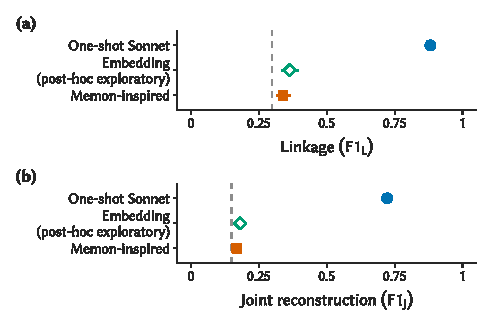
\includegraphics{fig1_headline_attackers.pdf}
  \caption{Headline prose, Game~J (46 pools). (a) Linkage component \FL;
  (b) joint \FJ. Means with $95\%$ percentile-bootstrap CIs over pools. The
  dashed line is the analytic one-bucket reference \bJ, which is a
  trivial-strategy benchmark rather than chance; a legal size-blind random
  seven-group answer scores $0.077$ (\S\ref{sec:baselines}). Open diamond:
  post-hoc exploratory attacker.}
  \label{fig:attackers}
\end{figure}
\input{table2_headline_attackers}
\input{table9_adjacency}

\subsection{Fragmentation strategy and granularity}
\label{sec:res-grid}
Across the nine retained conditions, \FJ{} ranged from $0.498$ (subject--verb
$\times$ clause) to $0.801$ (random $\times$ sentence); every cell sits well
above the analytic reference, the smallest advantage being $\AJ = 0.422$.
Subject--verb cuts were the most resistant at both granularities. Finer cuts
lowered \FJ{} modestly within three of the four strategies. At matched mean
fragment length the cutting strategy moved the result more than the granularity
label did.

\begin{figure}[t]
  \centering
  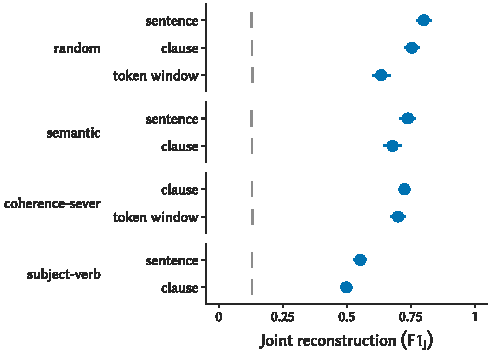
\includegraphics{fig2_grid_reconstruction.pdf}
  \caption{Game~J across the nine retained conditions and the full-length
  headline. (a) \FJ{} for the one-shot attacker ($95\%$ CI), Memon-inspired,
  the post-hoc embedding attacker and the analytic reference \bJ; (b)
  normalized advantage \AJ. One resource-bounded non-completion
  (random\,/\,token-window) is excluded and never scored $0$.}
  \label{fig:grid}
\end{figure}
\input{table3_grid}

\subsection{Linkage versus ordering}
\label{sec:res-decomp}
The decomposition separates which half each condition attacks. Subject--verb
cuts and random token windows act mainly on linkage; semantic-style boundaries
act mainly on ordering. The tested statistical attackers order at chance
throughout.

\begin{figure*}[t]
  \centering
  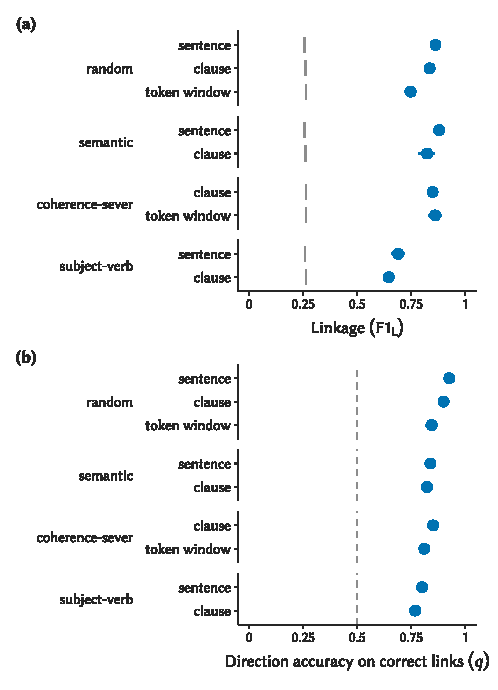
\includegraphics{fig3_linkage_vs_ordering.pdf}
  \caption{Decomposition of Game~J into (a) the linkage component \FL{} and
  (b) direction accuracy $q$ on the attacker's own correctly linked pairs;
  $\FJ=\FL\times q$ holds exactly per pool. The dotted line is chance for $q$.}
  \label{fig:decomp}
\end{figure*}

\subsection{Ordering when membership is given}
\label{sec:res-gameO}
With membership supplied, the one-shot attacker ordered the 100 full-length
headline documents at $\tau = 0.769$, i.e.\ $88.5\%$ of pairs correctly
ordered, with $\tau$ ranging from $0.724$ to $0.943$ across the grid cells. The
tested lexical orderers sat at chance. Contiguity on the same headline
documents was again much lower than the pairwise figure suggests: $32.5\%$ of
fragments in their exact position, a mean longest intact run of $6.31$
fragments, and a run fraction of $0.237$. Headline and grid results are
reported separately throughout and are not pooled; they move in opposite
directions in some comparisons. Full results are in
Appendix~\ref{app:gameO}.

\subsection{Structured identifiers}
\label{sec:res-identifiers}
The identifier arm behaved qualitatively differently. The one-shot attacker
scored $\FJ = 0.083$ $[0.068, 0.099]$ with $\FL = 0.132$---below the analytic
reference of $0.10$ and well below the truth-free schema-order baseline of
$0.20$. Its advantage over that baseline has a $90\%$ CI of
$[-0.162, -0.129]$: by the frozen rule this is not near the baseline, it is
below it. Every tested content-based attacker scored at or below the analytic
reference: Memon-inspired $0.054$, embedding $0.054$, random $0.056$.

What the attacker did recover was the template. All 140 groups contained
exactly one name, one SSN, one account number and one address, and $q = 0.631$
reflects that field-order regularity rather than record knowledge. Linkage
precision was $0.132$ against a template chance of $1/7$. In this synthetic arm
the schema structure remains directly exploitable while the tested
content-based attackers do not recover record association.

We state the inference carefully. Prose and identifiers differ in data type,
schema, fragment form and signal structure simultaneously, so this contrast is
consistent with reconstruction depending on the kind of signal the fragments
preserve; it does not isolate ``semantics'' as a causal variable. Nor does it
establish that identifier fragmentation is safe: it says that \emph{these}
attackers did not recover record association under \emph{this} setup
(\S\ref{sec:synthetic}).

\begin{figure}[t]
  \centering
  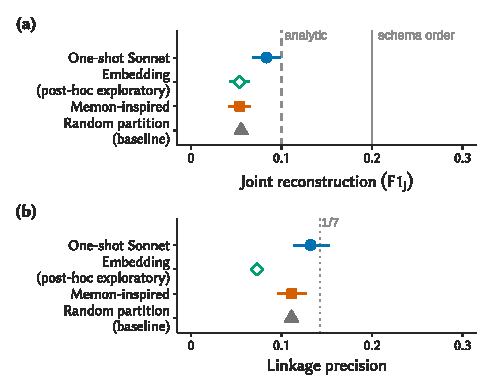
\includegraphics{fig4_identifiers.pdf}
  \caption{Synthetic identifiers, Game~J (20 pools of seven records). (a)
  \FL; (b) \FJ; (c) linkage precision, against the analytic ($0.10$ / $0.20$),
  schema-order ($0.20$) and template-chance ($1/7$) references. Open circles:
  the same attacker on the prose headline, for scale.}
  \label{fig:identifiers}
\end{figure}
\input{table5_identifiers}

\subsection{A controlled granularity series\posthoc}
\label{sec:res-gradient}
\textbf{This subsection is post-hoc exploratory.} It was designed after the
prespecified results were seen. On 20 headline pools and 140 four-sentence
excerpts, with byte-identical text in every arm and only the cut width
changing, we scored five granularities with the visible-text scorer and its
permutation null.

Null-adjusted joint reconstruction fell monotonically:
$\AVJ = 0.588$ (sentence), $0.350$ (4 words), $0.257$ (3 words), $0.127$
(2 words), $0.016$ (1 word). Two things must be read with it. The
random-shuffle reference is \emph{not} constant across arms---it falls from
$0.423$ at the sentence cut to $0.141$ at one word---so raw \VJ{} is not
comparable between arms and the normalized value is the one to read. And the
identifier-level score tracks the same shape but sits below it throughout.

\begin{figure}[t]
  \centering
  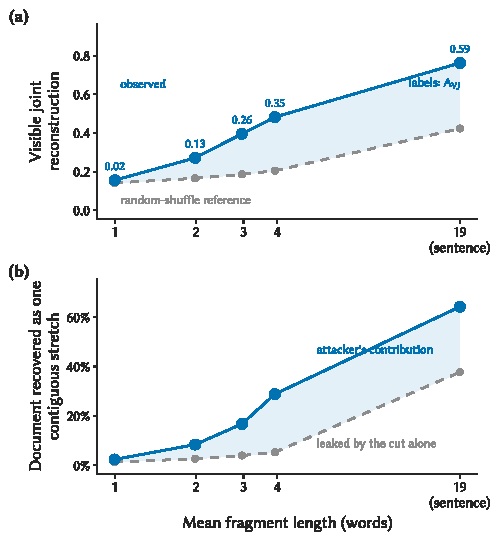
\includegraphics{fig6_granularity_gradient.pdf}
  \caption{Post-hoc exploratory granularity series: five cuts of identical
  text on the same 20 pools. (a) Observed \VJ{} against the random-shuffle
  reference for the same arm, which is not constant across arms; \AVJ{} is
  printed at each point. (b) Share of the 76-word excerpt recovered as one
  contiguous stretch, against the floor leaked by the cut alone. Join recall,
  which supports the two-regime reading, is $0.464$, $0.476$, $0.315$, $0.153$
  and $0.022$ from the sentence cut to one word.}
  \label{fig:gradient}
\end{figure}
\input{table8_gradient}

\paragraph{Two regimes.}
Panel~(b) separates what the cut gives away from what the attacker earns. At
the sentence cut the attacker ends up holding $64.2\%$ of the excerpt as one
contiguous stretch, but $37.7$ points of that are a single fragment, leaked
before any reconstruction happens. Between the sentence cut and the four-word
cut, join recall is essentially unchanged ($0.464$ versus $0.476$) while
contiguous recovery falls from $64.2\%$ to $28.8\%$: across that range the
reduction comes from the cut exposing less text per fragment rather than from
the attacker performing worse. Below four words, join recall itself declines
sharply---$0.315$, $0.153$, $0.022$---with contiguous recovery at $16.7\%$,
$8.4\%$ and $2.3\%$ and the corresponding floors at $3.9\%$, $2.6\%$ and
$1.3\%$.

In this controlled exploratory arm the transition occurs below roughly four
words: beyond that point the attacker's joining ability itself declines, rather
than privacy gains coming primarily from reducing the text each fragment
exposes. \textbf{Four words is not a universal threshold.} The arm uses one
corpus, one model, four-sentence excerpts and fixed-width word cuts, and is
post-hoc exploratory; the integer widths tested should not be interpolated.
This series extends the earlier binary sentence-versus-token edge case, which
is reported in Appendix~\ref{app:token}.

\subsection{Completion}
\label{sec:res-resources}
Of 652 prespecified one-shot units, 651 completed. The one unit that exhausted
its budget had 322 fragments, while units with as many as 537 fragments
completed elsewhere, and all post-hoc single-token units of up to 669
fragments completed---so fragment count is not a hard ceiling. It is reported in the
completion rate and never scored as zero. Output scaling and cost are in
Appendix~\ref{app:resources}.

% ===========================================================================
\section{Discussion}
\label{sec:discussion}
% ===========================================================================

\subsection{Why the generative attacker succeeds}
Similarity-based grouping reaches $\FL \approx 0.34$--$0.36$ on the same pools
where the one-shot attacker reaches $0.88$. The results are consistent with
fragment content providing a strong reconstruction channel---one that pairwise
lexical or embedding similarity does not capture. We did not run an experiment
that isolates which properties of the content carry that signal, so we do not
claim that entity continuity or chronology specifically were measured.

\subsection{Data-type dependence}
Prose fragments carry both linkage and ordering signal. Identifier fragments
carry a visible schema but, in this synthetic arm, no recoverable cross-record
association. In the controlled granularity series the joint structure falls to
its reference while some linkage signal persists. Resistance to reassembly, on
this evidence, is a property of the data type, the granularity, the attacker
and its budget, rather than of fragmentation alone. Disjointness did not remove
enough content signal to prevent substantial reconstruction in the prose
setting we tested.

\subsection{Implications for fragmentation as a privacy mechanism}
These results do not support treating plaintext fragmentation as a sole
confidentiality control for narrative text. They are consistent with it being,
at most, a data-dependent compromise-containment measure. For a practitioner
the two-regime finding of \S\ref{sec:res-gradient} is the usable part: in the
coarse range, finer cutting helps mainly by exposing less text per fragment,
because a sentence-sized fragment is a sentence of readable text whatever the
attacker does. We deliberately do not convert this into a recommended fragment
size.

\subsection{Limitations}
\label{sec:limitations}
\textbf{Closed world.} Complete pools, every fragment present, $N=7$ known, a
small pool. Deployment-level partial compromise, unknown source counts and
global populations are not evaluated.

\textbf{$N$ is fixed and unswept.} Neighbouring literatures vary the analogous
parameter---pool size and match prior in~\cite{lermen2026}, the number of mixed
documents in~\cite{paixao2020}---and we do not. How the result moves with $N$
is open, and results from a visual channel do not transfer to a semantic one.

\textbf{One corpus, one domain, one generative model.} English clinical case
reports and a single attacker model, with one embedding model.

\textbf{Tested attackers are not a frontier.} The Memon-inspired attacker is
not a faithful reproduction of the original algorithm, and the lexical
orderers run on a sparse similarity signal. Their results bound nothing about
what a stronger classical attacker could achieve.

\textbf{Post-hoc analyses.} The granularity series and the embedding attacker
were designed after results were seen and are labelled throughout. The series
uses four-sentence excerpts and fixed-width cuts, and locates no universal
threshold.

\textbf{References.} The analytic one-bucket benchmark is not a legal answer
and is roughly twice the legal random score, so advantages normalized against
it understate the margin (\S\ref{sec:baselines}).

\textbf{Confounds.} Context availability and search complexity move together
as granularity changes; the grid's granularity labels overlap in realised
fragment length; grid documents are capped at 30 sentences; and 21 headline
documents in 18 pools had documented development contact
(\S\ref{sec:pools}).

\subsection{Synthetic identifier data}
\label{sec:synthetic}
The identifier arm is evaluated entirely on synthetic records; no record
corresponds to a person. Its role is a contrast rather than an estimate: it
tests whether a content-based attacker that succeeds on prose also succeeds
when fragments carry schema regularities instead of narrative content. That
comparison depends on the \emph{structure} of the records---field types, field
order, format regularity---which the generator reproduces faithfully and which
is exactly what the schema-order baseline exploits. It does not depend on the
particular names or numbers, which is why synthetic values are adequate for
this purpose.

The arm does \emph{not} support any quantitative claim about real identifier
databases. Real records carry correlations between fields that a seeded
generator does not reproduce, and such correlations are precisely the kind of
dependency this paper shows can be exploited elsewhere. We therefore read this
result only as evidence that the tested attackers' advantage on prose does not
transfer to schema-dominated fragments. \TODO{authors: confirm this argument
satisfies the venue's synthetic-data requirement}

\subsection{Future work}
Global pools and unknown $N$; partial compromise; token-level attackers;
high-entropy secrets; other domains, languages and models; and a dedicated
mechanism experiment to identify which properties of content carry the
reconstruction signal.

% ===========================================================================
\section{Conclusion}
\label{sec:conclusion}
% ===========================================================================
Fragmentation removes explicit membership and order, but it does not
necessarily remove the relationships encoded in plaintext content. In a
closed-world clinical-prose setting, a modern generative attacker strongly
recovered source association and broad relative order, while immediate
adjacency and contiguous recovery remained much weaker. Reconstruction changed
sharply with the fragmentation regime and the data type, and in a controlled
post-hoc arm sufficiently fine fixed-width fragmentation drove the tested
attacker toward its random-shuffle reference. Resistance to reassembly is
therefore a property of the data, the granularity and the attacker, and
plaintext fragmentation should not be assumed to protect narrative text on its
own.

\appendix

\begin{acks}
Does NOT count towards page limit. NOT shown (as intended) for anonymous
submission. Only edit for the camera-ready. \TODO{funding; author
contributions; competing interests}
\end{acks}

% ---------------------------------------------------------------------------
\begin{ethics}
This study attacks documents that are already public and records that are
synthetic. The prose corpus consists of previously published, open-access
clinical case reports under commercial-use Creative Commons licences; we made
no attempt to identify any patient and add no information beyond the published
text. The identifier corpus is entirely synthetic, so no real identities,
account numbers or SSNs were involved and no attack on a real person is
possible. There is no human-subjects component and no interaction with people.

The capability we measure belongs to widely available models rather than to a
technique we introduce. We report it because designers of fragmentation schemes
cannot reason about a channel they have not been shown, and the direct
implication is defensive: plaintext fragmentation should not be relied on alone
for narrative text. We release what reproduces the study rather than packaged
attack tooling.

\TODO{state the model provider's data-use terms for API traffic; confirm
IRB/exempt status language and any institutional requirement}
\end{ethics}

% ---------------------------------------------------------------------------
\begin{openscience}
We release the measurement harness, the cutters and attackers, the scoring
code, the pool partitions, the frozen request specifications with their SHA-256
manifests, the dated decision log, the raw model outputs, the per-unit results,
and the figure and table scripts that regenerate every reported number. Each
figure ships the exact data frame it was plotted from, and the figure build
ends in an independent validation pass that checks every plotted value against
the frozen sources.

The prose corpus is reproducible from the published identifiers and the
retrieval scripts; redistribution of article text is subject to each article's
licence. The synthetic identifier corpus is reproducible from its seed. The
attacker is a proprietary API model, so responses are stored and every score
can be recomputed without re-querying; the embedding model is pinned by
revision and file hash.

\TODO{anonymized artifact URL for review; confirm the release licence and
whether fragment redistribution is permitted for every source article}
\end{openscience}

% ---------------------------------------------------------------------------
\begin{ai}
We distinguish between AI systems that are the subject of this study and AI
tools used to carry it out.

\emph{AI systems as objects of study.} The attackers we evaluate include a
generative large language model (\sonnet, accessed through the Message Batches
API) and a sentence-embedding model
(\textsf{sentence-transformers/all-mpnet-base-v2}, pinned to a fixed revision).
Their configuration, prompts and query protocol are described in
\S\ref{sec:attackers}, \S\ref{sec:protocol} and Appendix~\ref{app:prompts}.
During development we also queried other language models on development data
only; none contributes to a reported result. No model was fine-tuned.

\emph{AI assistance in conducting the research.} The authors used an AI coding
assistant throughout the project to write, test and debug the experiment and
analysis software; to audit code and intermediate results for errors; and to
draft internal documentation. \TODO{co-authors: state any AI assistance used in
your components; confirm assistant and model versions}

\emph{AI assistance in preparing the manuscript.} An AI assistant with access
to the project's decision log, frozen results and figure package produced a
complete reference draft, which the authors used to see one possible shape of
the argument before writing their own. The submitted manuscript is the authors'
own prose. The same assistant was used to check drafts for consistency with the
recorded design decisions and results and to flag passages needing
clarification. \TODO{authors: name any section that retains drafted text, or
state that none does}

\emph{Human oversight.} Every design decision, prespecification and
authorization of paid model queries was made by the authors and recorded in a
dated decision log released with the artifact. Analyses designed after results
were seen are labelled post hoc throughout. Every reported number is
regenerated by released scripts from the stored raw model outputs, and an
automated check verifies each quoted value against its source file. The authors
reviewed all code and text and take full responsibility for the content of this
paper. No AI system is listed as an author.
\end{ai}

\bibliographystyle{ACM-Reference-Format}
\bibliography{refs}

% ===========================================================================
% APPENDICES (outside the page limit; after the references)
% ===========================================================================
\section{Prompts}
\label{app:prompts}
Verbatim Game~J and Game~O prompts; alias format; parsing rule; repair feedback
text. \TODO{paste verbatim from the frozen specs}

\section{Full Grid Results and Paired Comparisons}
\label{app:grid}
Strategy and granularity paired tables; fragment mechanics per cell;
relationships between document length, fragment count and fragment size.

\section{Game O Details}
\label{app:gameO}
\begin{figure}[t]
  \centering
  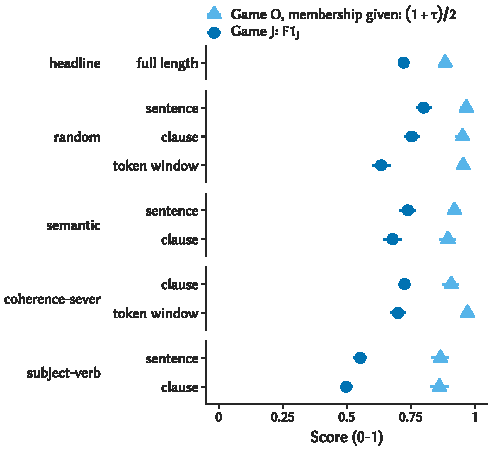
\includegraphics{figA_gameO_vs_gameJ.pdf}
  \caption{Ordering with membership given (Game~O, plotted as $(1+\tau)/2$)
  against joint reconstruction (Game~J \FJ{} and $q$) for the one-shot
  attacker. O: 100 headline documents, 30 per grid cell; J: 46 headline pools,
  24 (23) per cell. Game~O is a membership-oracle reference, not an upper bound
  on Game~J.}
  \label{fig:ovj}
\end{figure}
\input{table4_gameO}

\section{Completion, Resources and Cost}
\label{app:resources}
\begin{figure}[t]
  \centering
  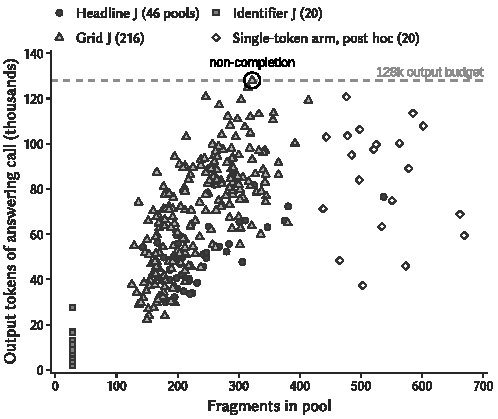
\includegraphics{figB_resource_scaling.pdf}
  \caption{Output tokens of the answering call against fragment count for every
  one-shot Game~J unit. The one resource-bounded non-completion (ringed) had
  322 fragments; the largest completed prespecified unit had 537, and all
  post-hoc single-token units of up to 669 fragments completed.}
  \label{fig:resources}
\end{figure}
\input{table7_resources}

\section{The Binary Single-Token Edge Case\posthoc}
\label{app:token}
Post-hoc exploratory. The same 20 headline pools and four-sentence excerpts cut
into sentences (28 fragments per pool) or single tokens: $\AVJ$ fell from
$0.588$ to $0.016$, a paired difference of $0.572$ $[0.539, 0.607]$, positive
in 20 of 20 pools, exact sign test $p = 1.9\times10^{-6}$, and robust to the
alternative null. Raw \VJ{} was $0.762$ against a null of $0.423$ at the
sentence cut and $0.155$ against $0.141$ at the token cut, while $\AVL$ fell
from $0.777$ to $0.159$: linkage signal survives where joint structure does
not. The binary design locates no threshold; \S\ref{sec:res-gradient} extends
it to five granularities.

\begin{figure}[t]
  \centering
  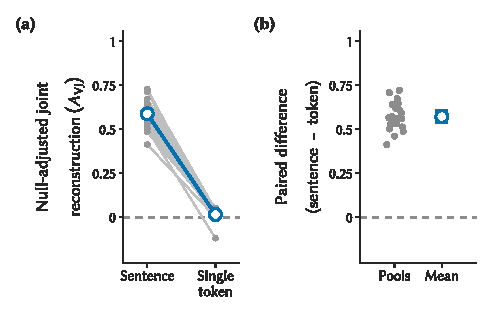
\includegraphics{fig5_single_token.pdf}
  \caption{Post-hoc exploratory single-token edge case.}
  \label{fig:token}
\end{figure}
\input{table6_single_token}

\begin{figure}[t]
  \centering
  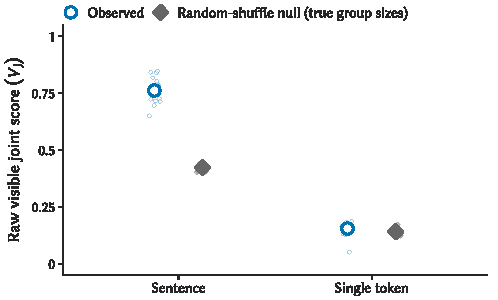
\includegraphics{figC_token_raw_vs_null.pdf}
  \caption{Post-hoc exploratory: observed against the null in raw terms.}
  \label{fig:rawnull}
\end{figure}

\section{Visible-Text Scorer, Nulls and Per-Pool Data}
\label{app:scorer}
Visible-text scorer definition and tests; permutation nulls (10{,}000 draws per
pool and condition); the predicted-structure robustness null; per-pool tables;
and results for the Memon-inspired and embedding attackers, which were not
designed for single-token input.

\section{Audits and Controls}
\label{app:audits}
The Jaccard orderer correction (an identifier-order leak via tie-breaking,
before and after); the masking side-channel control; the deterministic-seed fix
and reproducibility; and corpus fidelity checks.

\section{Development History and Screening}
\label{app:history}
Screening on a single pool and the dropped cells; the development-contact
inventory for the 21 documents in 18 headline pools; the synthetic-prose signal
inversion recorded during corpus construction; and the decomposed attacker that
was designed but not run.

\end{document}
